
The design of fast algorithms for (\ref{gt}) is strongly dependent on three independent parameters viz., the number of sources $N$, the bandwidth $\delta$ and desired accuracy $\epsilon$. A Gaussian centered at a source location interacts with targets that are within its support. If there are fewer targets than a threshold value $n^*$, we use a simple {\em truncation algorithm}, otherwise, we use a {\em expansion algorithm}. The threshold  value depends on all three independent parameters and we will discuss its choice after introducing both algorithms. 

\subsection{Truncation algorithm} 
Since the kernel in (\ref{gt}) decays exponentially, we can simply truncate the sum to
%
\beq F(x_j) = \sum_{y_k \in \mathcal{I}[x_j]} \kernel f(y_k) \label{eqn:truncation} \eeq
%
where $\mathcal{I}[x_j]$ is the interaction list which includes all the sources that are within a distance $\sqrt{\delta \ln (\frac{1}{\epsilon})}$. Beyond this distance, a Gaussian centered at $x_j$ decays below $\epsilon$. The complexity of this algorithm is $\bigO(N \sqrt{\delta \ln(\frac{1}{\epsilon})})$. This is a common technique used in the graphics community (Gaussian blurring). When $\delta$ is large and/or high accuracy is required, the cost of this algorithm grows quadratically.  

\subsection{Expansion algorithm}
Broadly speaking, FGT algorithms \cite{fgt, greengard98} partition the domain into boxes of uniform size and proceed in three main steps: (i) compress the influence of sources into a few multipole-type moments, (ii) translate the moments across the domain and (iii) evaluate the moments at the targets. In the original FGT \cite{fgt}, the translation costs tend to dominate \cite{fggt}. The plane-wave expansion version \cite{greengard98} minimized the translation costs to a large extent but at the expense of higher computational cost for steps (i) and (iii). This problem is alleviated in \cite{fggt} to a large extent. Our implementation is based on \cite{fggt} and we summarize it here. 

Central to the expansion algorithm is the finite-term plane-wave expansion of the kernel,
\beq G_\delta(\norm{x_j - y_k}) \approx \sum_{|k| \leq p} \hat{G}(k) e^{i \lambda k \cdot (x_j - y_k)}, \quad \lambda = \frac{L}{p\sqrt{\delta}}\eeq
where $k = (k_1, k_2, k_3)$ and the parameters $p$ and $L$ are determined by the required precision. $\hat{G}$ is the discrete Fourier transform of the kernel. For the Gaussian kernel, it is given by
\beq \hat{G}(k) = \left(\frac{L }{2p\sqrt{\pi}}\right)^3 e^{-\frac{\lambda^2 |k|^2 \delta}{4}}. \label{eqn:ghat}\eeq

The algorithm begins by partitioning the domain into uniform boxes of size $\sqrt{\delta}$ each. A Gaussian located at the center of a box $B$ decays below $\epsilon$ beyond a fixed number of boxes. We call these boxes the interaction list of $B$, denoted by $\mathcal{I}[B]$. 

In the fast algorithm, a target point $x \in D$ receives information from a source point $y \in B$ in three steps:
\begin{description}
\item[\textbf{S2W}] The influence of all the sources in the box $B$ is condensed into a plane-wave expansion:
            \beq w_k = \sum_{y \in B} f(y) e^{i\lambda k \cdot (c^B - y)} \quad \forall\quad |k| \leq p  \label{eqn:s2w} \eeq
            
\item[\textbf{W2L}] The plane-wave expansion of each box $B$ is transmitted to every box $D$ in $\mathcal{I}[B]$. By
 superposition, the ``local'' plane-wave expansion of $D$ gets modified as
            \beq v_k += w_k e^{i\lambda k \cdot (c^D - c^B)} \label{e:w2l}\eeq
            
\item[\textbf{L2T}] The transform (\ref{gt}) is computed at each target by evaluating the local expansion of the 
box it is contained in:
            \beq F(x) = \sum_{|k| \leq p} \hat{G}(k) v_k e^{i\lambda k \cdot (x - c^D)} \label{eqn:l2t}\eeq
\end{description} 

First, the S2W step is executed seperately in each box with $\bigO(p^3 N)$ work. In a {\em direct scheme}, 
the W2L is executed by simply visiting each box $B$ and translating its plane-wave expasion to all the boxes
 in $\mathcal{I}[B]$. Assuming the size of interaction list is $K^3$, this algorithm requires $\bigO(K^3 p^3 |B|)$ work 
 to form local expansions at all the boxes. Finally, the L2T is executed by visiting each box and evaluating the 
 local expansion at the targets, requiring $\bigO(p^3 N)$ work. Therefore, the overall cost of the algorithm is $\bigO(p^3 N + K^3 p^3 |B|)$.  

\subsection{Overall algorithm} 
The translation costs can be reduced dramatically by using the {\em sweeping algorithm} introduced in \cite{greengard98}. We present a 
modified version of the same in Section \ref{sc:sweep}. The total cost of the expansion algorithm is then typically dominated by the S2W
 and L2T steps. If the points within each FGT box lie on a tensor-product grid, then we incorporate the accelerations described in \cite{fggt}. With these
 accelerations, the cost of the S2W and L2T steps reduces to $\bigO(p^3 N^{\frac{1}{3}})$.
 However, when $\delta$ is lower and/or $\epsilon$ is higher, the cost of the expansion algorithm increases because 
 condensing the sources into plane-waves becomes increasingly futile as the number sources per box gets reduced. On the other hand, the
 cost of the truncation algorithm decreases. Hence, we choose between the two algorithms based on the following heuristic:

{\tt
\begin{algorithmic}
\STATE
  \IF {$N \sqrt{\delta \ln \left( \frac{1}{\epsilon} \right)} < (2p)^3 $}
     \STATE Use truncation algorithm 
  \ELSE 
     \STATE Use expansion algorithm
  \ENDIF
\STATE
\end{algorithmic}
}

\begin{figure}
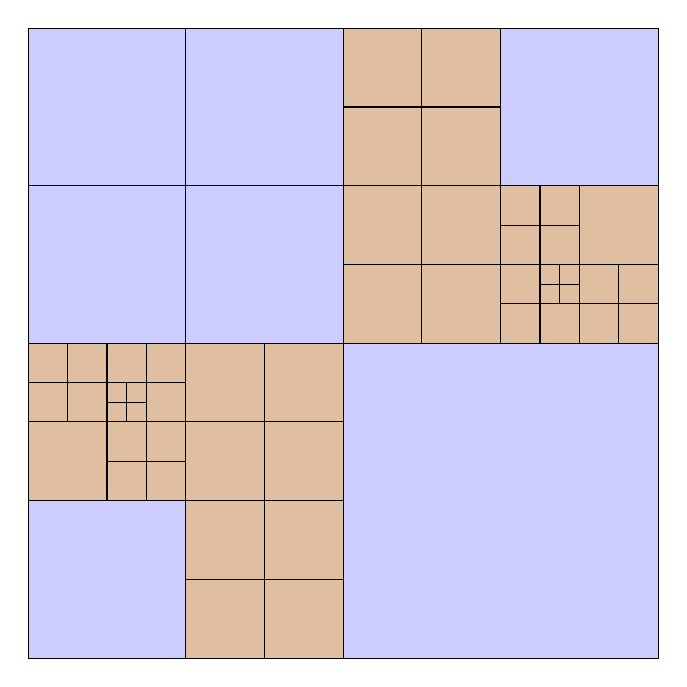
\begin{tikzpicture}[scale=0.5]

\draw[fill=blue!20] (0,8) rectangle +(8,8);
\draw[fill=blue!20] (8,0) rectangle +(8,8);
\draw[fill=blue!20] (0,0) rectangle +(4,4);
\draw[fill=blue!20] (12,12) rectangle +(4,4);

\draw[fill=brown!50] (4,0) rectangle +(4,4);
\draw[fill=brown!50] (0,4) rectangle +(4,4);
\draw[fill=brown!50] (4,4) rectangle +(4,4);
\draw[fill=brown!50] (8,8) rectangle +(4,4);
\draw[fill=brown!50] (8,12) rectangle +(4,4);
\draw[fill=brown!50] (12,8) rectangle +(4,4);



%Draw the initial octree
\draw[step = 8] (0,0) grid (16,16);
\draw[step = 4] (8,8) grid(16,16);
\draw[step = 4] (0,8) grid(8,16);
\draw[step = 2] (0,4) grid(4,8);
\draw[step = 2] (4,4) grid (8,8);
\draw[step = 2] (4,0) grid (8,4);
\draw[step = 1] (2,4) grid (4,8);    	
\draw[step = 1] (0,6) grid (2,8);
\draw[step = 0.5] (2,6) grid (3,7);

\draw[step = 2] (8,8) grid(12,16);
\draw[step = 2] (12,8) grid (16,12);
    	    	
\draw[step = 1] (12,8) grid (14,12);
\draw[step = 1] (14,8) grid (16,10);
\draw[step = 0.5] (13,9) grid (14,10);    	    	    	    	
    	    	    	    	
\end{tikzpicture}
\caption{Truncation or Expansion ? }  
\end{figure}

%\subsection{Kernel independence} 
%The advantage of the plane-wave expansion (\ref{eqn:ghat}) is that once  
%If the kernel values are known at the discrete points $\{Lk/p \}_{|k| \leq p}$, then we can compute $\hat{G}$ using discrete Fourier transform. 

\subsection{Parallel truncation algorithm}
We divide the unit cube into a regular grid of boxes and distribute the boxes across $n_p$ processors
 such that {\tt{(a)}} each processor owns exactly one box and {\tt{(b)}} each box is owned by an unique processor.
 For each source owned by this processor, we find out the processors that contain boxes which intersect the interaction list
 for that source and send the source to those processors. Each processor then evaluates (\ref{eqn:truncation}) for all its targets.
 
\subsection{Parallel expansion algorithm} 
We create a regular grid of $|B|$ FGT boxes distributed on $n_p$ processors 
such that {\tt{(a)}} each box is owned by an unique processor and {\tt{(b)}} each processor owns a 
sub-grid of FGT boxes. For ease of implementation, we assume that $|B| > n_p$. 
 We use PETSc's \cite{petsc-user-ref, petsc-home-page} DA module to manage this distributed regular grid.
 The S2W and L2T steps are embarassingly parallel; in the former step, each processor independently forms the 
 plane-wave expansions for each box that it owns and in the latter step, each processor
 independently computes the transform (\ref{gt}) for each target contained within some box owned by
  that processor using the local expansion for that box. Hence, the cost for these two steps is 
  simply $\bigO(p^3 \frac{N}{n_p})$. For the W2L step, each processor first gathers the plane-wave expansions of
  the boxes that are in the interaction list of some box owned by that processor. The communication cost for
  this step is $\bigO(K (\frac{|B|}{n_p})^{\frac{2}{3}} + K^2(\frac{|B|}{n_p})^{\frac{1}{3}} + K^3 )$.
Following this communication, each processor executes the sequential W2L algorithm for all boxes that it owns. 
 If we use the direct scheme for the sequential W2L algorithm then this cost would be $\bigO(p^3 K^3 \frac{|B|}{n_p})$.
 As mentioned earlier, this cost can be reduced by using the sweeping algorithm, which is described in the following section. 


